En el camino de la creación de robots hasta este momento se habían diseñado pensando siempre en su aplicación empresarial o industrial. ASIMO pudo ser el primero en el que la gente se pudiera replantear su utilidad dentro de una casa para cumplir tareas sencillas, pero debido a su alto precio (incluso no fueron comercializados más allá de hacer demostraciones para empresas) no eran accesibles a nadie o casi nadie. En este punto surgió la compañía iRobot Corporation, una compañía fundada por tres ingenieros del MIT: Rodney Brooks, Colin Angle y Helen Greiner quienes venían de trabajar y estudiar en el Laboratorio de Inteligencia Artificial del MIT.

iRobot cambió un poco la perspectiva de las personas al hacer que se incluyeran en casa robots de un precio asequible cuyas aplicaciones reales eran verdaderamente útiles (no como un asistente ASIMO en una casa).

La compañía fue fundada en 1990, época por la cual trabajaban con robots aplicados a la tecnología militar, como fue su robot PackBot usado en las guerra de Iraq y Afghanistan como apoyo a las tropas. El robot era útil puesto que incorporaba un sistema que le permitía superar obstáculos tales como piedras, escaleras, huecos, etc gracias a las orugas con las que se desplazaba. iRobot además no sólo tuvo contratos con la industria militar si no que, además, mantuvo relaciones con la NASA desarrollando robots para ellos también.

Tras los contratos mencionados anteriormente iRobot comenzó su andadura en los robots de ámbito doméstico con robots dedicados a la limpieza y ampliamente conocidos: los Roomba, Braava y Mirra. De aquí los más conocidos son los del modelo Roomba. Este robot actualmente es capaz de barrer y fregar una casa de forma autónoma y aunque nos parezca trivial o de poca relevancia no lo es en absoluto. Estos robots incorporan todo el desarrollo de los mencionados anteriormente, no sólo la capacidad de moverse y limpiar, si no también la capacidad de aprender de su entorno haciendo un mapa de las habitaciones, ser capaz de esquivar obstáculos y recalcular su trayectoria, así como la capacidad de volver al punto de donde partió (su base de carga). Este modelo en concreto es un hito en la historia de la robótica al traer a casa tecnología muy avanzada en cuestión de robótica y domótica a un precio más asequible que los robots diseñados hasta el momento.

\begin{figure}[!h]
	\centering
	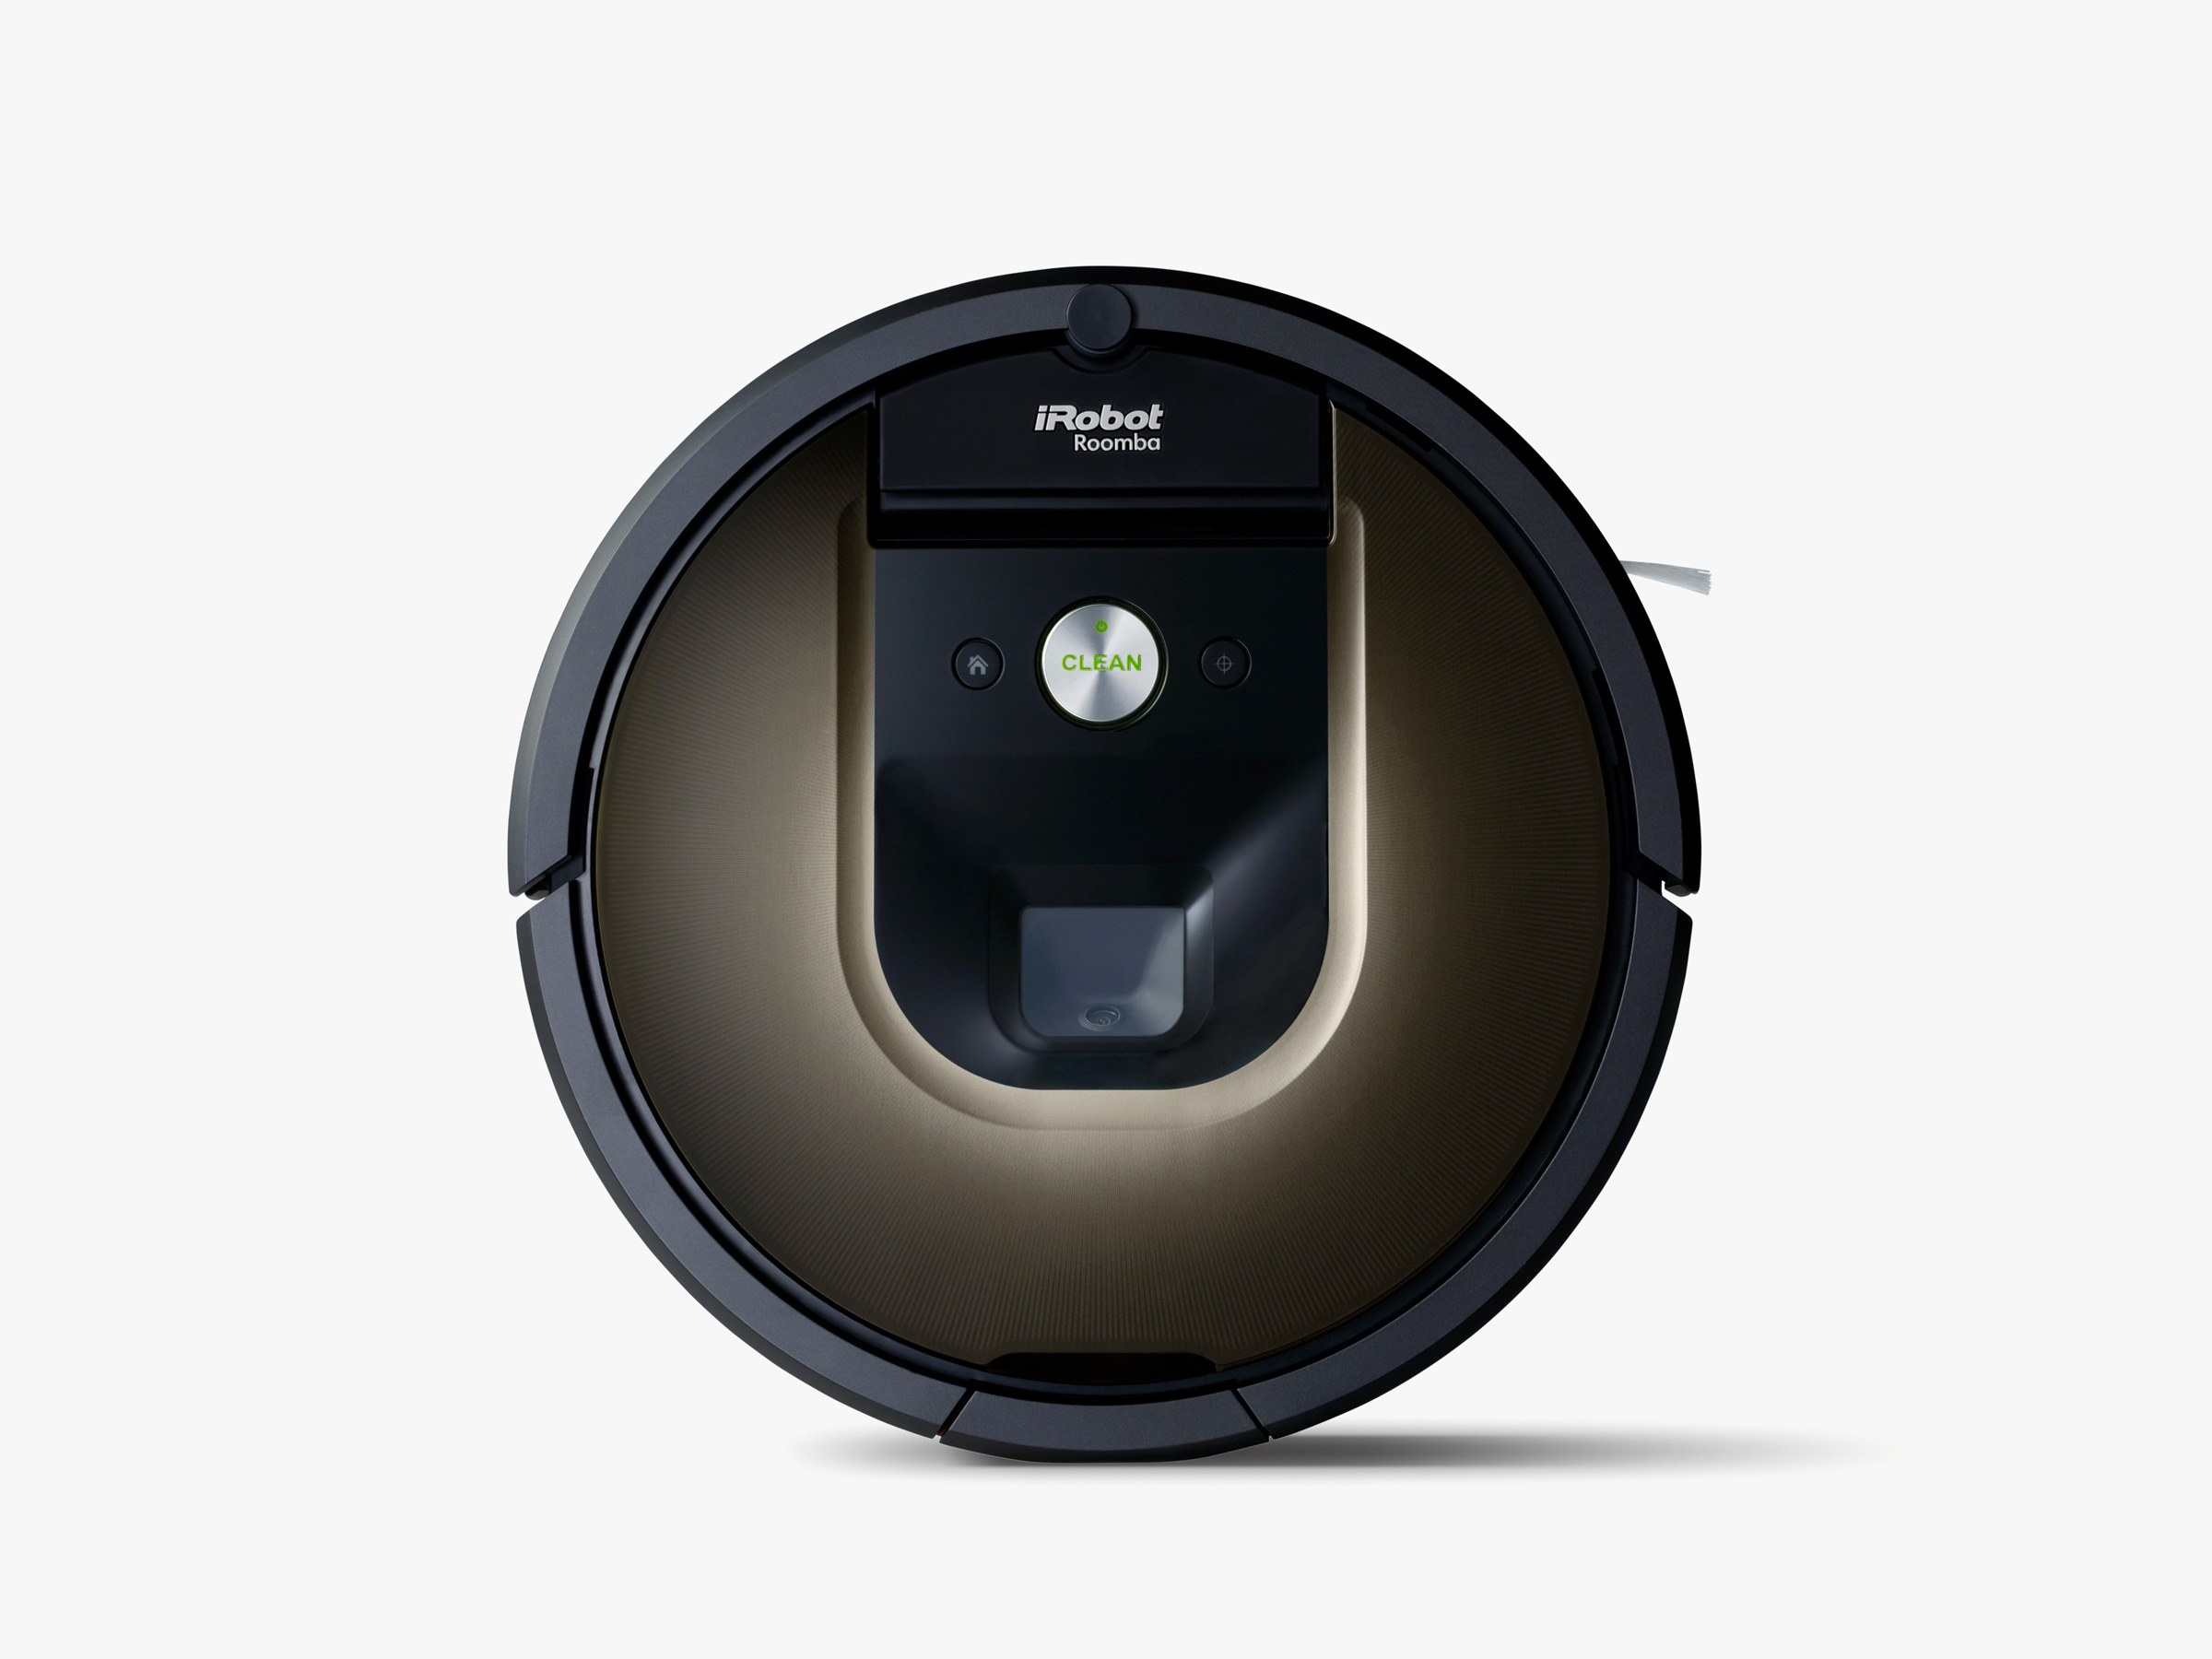
\includegraphics[scale=0.1]{./EtapaModerna/Imagenes/roomba.jpg}
	\caption{Roomba (\href{https://commons.wikimedia.org/wiki/File:IRobot\_Roomba\_980.jpg}{Wikimedia})}
	\label{fig:roomba}
\end{figure}